\documentclass{beamer}

\usepackage{polski}
% Add TikZ package for drawing graphs
\usepackage{tikz}

\usetheme{metropolis}
\title{Markow Decision Processes and Reinforcement Learning}
\author{K. Drozd, M. Zięć}
\institute{Uniwersytet Jagielloński w Krakowie}
\date{\today}

% Define auxilliaty aliases
\newcommand{\Natural}{\mathbb{N}}
\newcommand{\Real}{\mathbb{R}}
\newcommand{\State}{\mathbb{S}}
\newcommand{\Action}{\mathbb{A}}

\begin{document}

\begin{frame}
    \titlepage
\end{frame}

\begin{frame}{Outline}
    \tableofcontents
\end{frame}



\section{Markow Decision Processes}
\subsection{Introduction}
\begin{frame}{Markow Decision Process}
    \centering
    discrete time Markow Process:\\
    Stochstic Process $X_t$, $t \in \Natural$ admitting the \textbf{Markow Proprety}.
    
    (discrete) state space $ \State \ni s $

    transition probability $ P[X_{t+1} = s' \mid X_t = s] $

    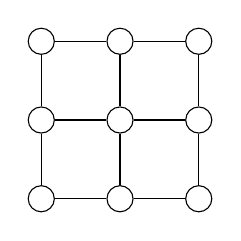
\begin{tikzpicture}[scale=1]
        % Draw nodes
        % Draw nodes explicitly
        \node[circle,draw,fill=white] (n00) at (0,0) {};
        \node[circle,draw,fill=white] (n01) at (0,1) {};
        \node[circle,draw,fill=white] (n02) at (0,2) {};
        \node[circle,draw,fill=white] (n10) at (1,0) {};
        \node[circle,draw,fill=white] (n11) at (1,1) {};
        \node[circle,draw,fill=white] (n12) at (1,2) {};
        \node[circle,draw,fill=white] (n20) at (2,0) {};
        \node[circle,draw,fill=white] (n21) at (2,1) {};
        \node[circle,draw,fill=white] (n22) at (2,2) {};

        % Draw horizontal edges explicitly
        \draw (n00) -- (n10);
        \draw (n10) -- (n20);
        \draw (n01) -- (n11);
        \draw (n11) -- (n21);
        \draw (n02) -- (n12);
        \draw (n12) -- (n22);

        % Draw vertical edges explicitly
        \draw (n00) -- (n01);
        \draw (n01) -- (n02);
        \draw (n10) -- (n11);
        \draw (n11) -- (n12);
        \draw (n20) -- (n21);
        \draw (n21) -- (n22);
    \end{tikzpicture}
\end{frame}

\begin{frame}{Markow Decision Process}
    \centering
    discrete time Markow \textbf{Decision} Process:\\
    Agent which can take \textbf{actions} $a \in \Action(s)$ where $s \in \State$.\\
    Feedback is given via \textbf{reward} $r \in \Real$

    transition probability $ P[X_{t+1} = s', R_{t+1} = r \mid X_t = s, A_t = a] $\\
    Maximise expected reward: 
    \[ \text{E}\left[\sum \limits_{t=0}^{\infty} R_t\right] \]
    
    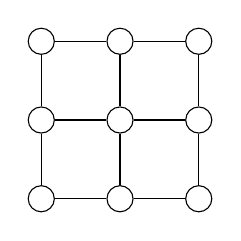
\begin{tikzpicture}[scale=1]
        % Draw nodes
        % Draw nodes explicitly
        \node[circle,draw,fill=white] (n00) at (0,0) {};
        \node[circle,draw,fill=white] (n01) at (0,1) {};
        \node[circle,draw,fill=white] (n02) at (0,2) {};
        \node[circle,draw,fill=white] (n10) at (1,0) {};
        \node[circle,draw,fill=white] (n11) at (1,1) {};
        \node[circle,draw,fill=white] (n12) at (1,2) {};
        \node[circle,draw,fill=white] (n20) at (2,0) {};
        \node[circle,draw,fill=white] (n21) at (2,1) {};
        \node[circle,draw,fill=white] (n22) at (2,2) {};

        % Draw horizontal edges explicitly
        \draw (n00) -- (n10);
        \draw (n10) -- (n20);
        \draw (n01) -- (n11);
        \draw (n11) -- (n21);
        \draw (n02) -- (n12);
        \draw (n12) -- (n22);

        % Draw vertical edges explicitly
        \draw (n00) -- (n01);
        \draw (n01) -- (n02);
        \draw (n10) -- (n11);
        \draw (n11) -- (n12);
        \draw (n20) -- (n21);
        \draw (n21) -- (n22);
    \end{tikzpicture}
\end{frame}


\subsection{Solving MDPs}
\subsubsection{Transition Probabilities Known}
\subsubsection{Given Data Incomplete}

\end{document}